\documentclass[10pt,twocolumn,letterpaper]{article}

% Meine eigenen Sachen
\usepackage{booktabs}
% \usepackage{caption}
% \captionsetup[table]{skip=8pt}   % Betrifft nur Tabellen
\usepackage{stfloats}  % Fügt dies dem Vorspann hinzu
\usepackage{float}
\usepackage[T1]{fontenc}
\usepackage[utf8]{inputenc}  % Stellt UTF-8 Codierung sicher

\usepackage{cvpr}
\usepackage{times}
\usepackage{epsfig}
\usepackage{graphicx}
\usepackage{amsmath}
\usepackage{amssymb}

% Weitere Pakete hier einfügen, vor hyperref.

% Wenn hyperref auskommentiert und dann wieder einkommentiert, solltest du
% egpaper.aux löschen, bevor Latex erneut ausgeführt wird. (Oder einfach beim ersten Latex 'q' drücken.)
% ausführen, laufen und beenden lassen, und das sollte passen
\usepackage[breaklinks=true,bookmarks=false]{hyperref}

\cvprfinalcopy % *** Diese Zeile für die letztendliche Einreichung unkommentieren

\def\cvprPaperID{****} % *** Die CVPR Paper ID hier einfügen
\def\httilde{\mbox{\tt\raisebox{-.5ex}{\symbol{126}}}}

% Seiten sind im Einreichungsmodus nummeriert und in der endgültigen Version unnummeriert
%\ifcvprfinal\pagestyle{empty}\fi
\setcounter{page}{1}
\begin{document}

%%%%%%%%% TITEL
\title{ECDO Datengetriebener Leitfaden Teil 1/2: Aktueller Stand des Verständnisses der exothermen Kern-Mantel-Entkopplung Dzhanibekov-Oszillation (ECDO) “Earth Flip” Theorie}

\author{Junho\\
Veröffentlicht im Februar 2025\\
Webseite (Papiere hier herunterladen): \href{https://sovrynn.github.io}{sovrynn.github.io}\\
ECDO Forschungs-Repo: \href{https://github.com/sovrynn/ecdo}{github.com/sovrynn/ecdo}\\
{\tt\small junhobtc@proton.me}
% Für eine Arbeit, deren Autoren alle an derselben Institution sind,
% lass die folgenden Zeilen bis zur schließenden ``}'' weg.
% Weitere Autoren und Adressen können mit ``\and'' hinzugefügt werden,
% genauso wie der zweite Autor.
% Um Platz zu sparen, verwende entweder die E-Mail-Adresse oder die Homepage, nicht beides
% \und
% xxx
% Institution2\\
% Erste Zeile der Adresse von Institution2\\
% {\tt\small secondauthor@i2.org}
}

\maketitle
%\thispagestyle{empty}

%%%%%%%%% ABSTRAKT
\begin{abstract}
Im Mai 2024 teilte ein pseudonymer Online-Autor mit dem Namen „The Ethical Skeptic“ \cite{0} eine bahnbrechende Theorie namens Exothermic Core-Mantle Decoupling Dzhanibekov Oscillation (ECDO) \cite{1}. Diese Theorie legt nahe, dass die Erde in der Vergangenheit plötzliche, katastrophale Verschiebungen ihrer Rotationsachse erlebt hat, die massive weltweite Überschwemmungen auslösten, als die Ozeane aufgrund der Rotationsträgheit über die Kontinente schwappten. Darüber hinaus präsentiert sie einen erklärenden geophysikalischen Prozess und Daten, die darauf hinweisen, dass ein weiterer solcher Umsturz unmittelbar bevorstehen könnte. Obwohl katastrophale Flut- und Weltuntergangsprognosen nicht neu sind, ist die ECDO-Theorie aufgrund ihres wissenschaftlichen, modernen, multidisziplinären und datenbasierten Ansatzes besonders überzeugend.

Diese Arbeit ist der erste Teil einer zweiteiligen komprimierten Zusammenfassung von sechs Monaten unabhängiger Forschung \cite{2,20} zur ECDO-Theorie. Sie hebt drei Schlüsselpunkte hervor:

\begin{flushleft}
\begin{enumerate}
    \item Eine ECDO-ähnliche „Erdumdrehung“ hat sich in der jüngeren Menschheitsgeschichte mehrfach ereignet, wie Flutmythen und geologische Anzeichen weit verbreiteter kontinentaler Überschwemmungen belegen.
    \item Die ungefähre Richtung und Stärke vergangener Erdumdrehungen können bestimmt werden.
    \item Aktuelle geomagnetische und geophysikalische Daten deuten darauf hin, dass eine weitere Erdumdrehung bevorstehen könnte und dass der Klimawandel eher durch Veränderungen tief im Erdinneren als durch den Menschen verursacht werden könnte.
\end{enumerate}
\end{flushleft}

Zusätzlich erläutere ich die zugrunde liegende Physik einer durch die ECDO-Theorie vorgeschlagene „Erdumdrehung“.

In dieser Arbeit bleibe ich objektiv, indem ich mich auf harte Daten konzentriere, überzeugende, aber spekulative Teile der Theorie vermeide und betone, dass dies ein Thema ist, das die Menschheit dringend weiter untersuchen muss.
\end{abstract}

%%%%%%%%% BODY-TEXT
\section{Einleitung}

Geschichten von einer großen Flut sind nicht neu – tatsächlich finden sie sich in jeder bedeutenden Kultur rund um den Globus und durchziehen alle Wiegen der Zivilisation. Eine Zusammenstellung von 267 Flutgeschichten \cite{3}, dargestellt in Abbildung \ref{fig:1}, zeigt, dass praktisch alle bewohnten Regionen der Erde Flutgeschichten enthalten.
```latex
% \begin{figure}[h]
% \begin{figure}[b]
\begin{figure}[h]
\begin{center}
% \fbox{\rule{0pt}{2in} \rule{0.9\linewidth}{0pt}}
   \includegraphics[width=1\linewidth]{b.png}
\end{center}
   \caption{Standorte von Flutgeschichten auf der ganzen Welt \cite{3}.}
\label{fig:1}
\label{fig:onecol}
\end{figure}

Ein genauerer Blick auf diese Flutgeschichten zeigt uns, dass es sich hierbei nicht um gewöhnliche Überschwemmungen handelte, sondern um zerstörerische Katastrophen, die von Fluten begleitet wurden, welche die Kontinente vollständig betroffen haben.

\subsection{Katastrophengeschichten der amerikanischen Ureinwohner}

Geschichten der amerikanischen Ureinwohner enthalten einige der anschaulichsten Berichte über die großen Katastrophen der Erde. Die Hopi, ein Stamm amerikanischer Ureinwohner, der im Nordosten Arizonas lebt, sagen, dass, \textit{"..Sótuknang die Ameisenmenschen aufforderte, ihre unterirdische Welt für das auserwählte Volk zu öffnen. Als sie sicher unter der Erde waren, befahl Sótuknang den Zwillingen, Pöqánghoya und Palöngawhoya, ihre Posten an den nördlichen und südlichen Enden der Erdachse zu verlassen, wo sie stationiert waren, um die Erde ordnungsgemäß rotieren zu lassen. \textbf{Die Zwillinge hatten kaum ihre Posten verlassen, als die Welt, ohne jemanden, der sie kontrollierte, aus dem Gleichgewicht geriet, sich verrückt drehte und dann zweimal überschlug.} Berge stürzten mit einem gewaltigen Platschen ins Meer, Meere und Seen schwappten über das Land; und als die Welt durch den kalten und leblosen Raum wirbelte, fror sie zu festem Eis."} \cite{4}.

Viele dieser Geschichten beschreiben präzise das gewaltige Ausmaß der Überschwemmungen und berichten davon, wie die Ozeane anstiegen, um alles außer den höchsten Berggipfeln zu überfluten. Die Skokomish-Indianer, die im Bundesstaat Washington leben, erzählen, wie, \textit{"Der Große Geist, zornig über die Bosheit der Menschen und Tiere, beschloss, die Erde von allen außer den guten Tieren, einem guten Mann und seiner Familie zu befreien. Auf Anweisung des Großen Geistes schoss der Mann einen Pfeil in eine Wolke, dann einen weiteren Pfeil in diesen Pfeil, und so weiter, wobei er ein Seil aus Pfeilen von der Wolke zum Boden herstellte. Die guten Tiere und Menschen kletterten hinauf. Böse Tiere und Schlangen begannen hinaufzuklettern, aber der Mann riss das Seil ab. \textbf{Dann ließ der Große Geist viele Tage Regen fallen, der bis zur Schneegrenze von Takhoma (Mount Ranier) überschwemmte.} Nachdem alle bösen Menschen und Tiere ertrunken waren, stoppte der Große Geist den Regen, das Wasser sank langsam, und die guten Menschen und Tiere kletterten wieder hinunter."} \cite{3}. Zum Vergleich: Der Mount Rainier ist ein aktiver Vulkan im Bundesstaat Washington mit einer Gipfelhöhe von 4392,5 m über dem Meeresspiegel.
```
The Flutgeschichte der Makah-Indianer aus dem US-Bundesstaat Washington erwähnt ausdrücklich eine mehrphasige Flut von „sehr warmem“ Wasser, was darauf hindeutet, dass dies keine normale Flut war: \textit{„Der Ozean stieg so hoch, dass das Kap abgeschnitten wurde. Dann zog er sich zurück und erreichte seinen niedrigsten Stand vier Tage später, wobei Neah Bay hoch und trocken blieb. Dann stieg er wieder an und bedeckte alles bis auf die Berggipfel. \textbf{Das aufsteigende Wasser war sehr warm.} Menschen mit Kanus luden ihre Habseligkeiten ein und wurden weit nach Norden getragen. Viele starben, als ihre Kanus in Bäumen hängen blieben. Das Meer kehrte nach weiteren vier Tagen zur Normalität zurück, und die Menschen fanden sich weit im Norden wieder, wo ihre Nachfahren noch immer wohnen“} \cite{3}.

\subsection{Chinesische Katastrophenberichte}

Auf der anderen Seite des Pazifiks soll die moderne chinesische Zivilisation mit einer großen Flut begonnen haben. Die Xia-Dynastie, die auf etwa 2000 v. Chr. datiert wird, wurde von Yu dem Großen gegründet, der die Große Flut von Gun-Yu beendete \cite{6}. In seiner Zeit geschah \textit{„...das Wunder, dass die Sonne zehn Tage lang nicht unterging, die Wälder in Brand gerieten und eine Vielzahl abscheulicher Ungeheuer hervorgebracht wurden... Eine riesige Welle, „die den Himmel erreichte“, stürzte auf das Land China herab. \textbf{„Das Wasser stand hoch bis auf die Berge, und die Vorgebirge waren überhaupt nicht mehr zu sehen“}... „Vernichtend in ihrem Überlauf sind die Wasser der Überschwemmung“, sagte der Kaiser. „In ihrer riesigen Ausdehnung umschließen sie die Hügel und übersteigen die großen Höhen, drohen mit ihren Fluten dem Himmel.“ Der Kaiser befahl, dass alle Anstrengungen unternommen werden sollten, um Auslässe für das Wasser zu schaffen, das sich in den Tälern zwischen den Bergen gesammelt hatte. Viele Jahre lang arbeiteten die Menschen daran, die Ebenen und Täler vom Wasser der Flut zu befreien, indem sie Kanäle gruben und Felder entwässerten. Lange Jahre war alle Mühe vergeblich. Der Minister, der für diese dringende und gewaltige Aufgabe verantwortlich war, Khwan, wurde aufgrund seines Scheiterns zum Tode verurteilt... und erst sein Sohn Yu hatte Erfolg bei der Trockenlegung des Landes. Diese Leistung wurde so hoch eingeschätzt, dass Yu nach König Shun, dem ersten Nachfolger Yahous, Kaiser von China wurde“} \cite{5}.

Es scheint, dass nicht nur China überflutet wurde, sondern dass es notwendig war, die Himmelsrichtungen sowie die Bewegungen von Sonne und Mond neu zu bestimmen, was darauf schließen lässt, dass sich während der Flut die Erdrotation verändert haben könnte: \textit{\textbf{„Dieser Kaiser sandte Gelehrte in verschiedene Teile Chinas und sogar nach Indochina, um die Lage von Norden, Westen, Osten und Süden durch Beobachtung des Sonnenaufgangs, Sonnenuntergangs und der Bewegung der Sterne herauszufinden.} Er beauftragte auch seine Astronomen, die Dauer der Jahreszeiten zu bestimmen und einen neuen Kalender zu erstellen... „Daraufhin befahl Yaou [Yahou] He und Ho, in ehrfürchtigem Einklang mit dem weiten Himmel die Bewegungen und Erscheinungen von Sonne, Mond, Sternen und Tierkreisräumen zu berechnen und zu beschreiben und den Leuten die Jahreszeiten mitzuteilen“"} \cite{5}.

Berichte über Katastrophen in der chinesischen Geschichte reichen tatsächlich weit vor die Xia-Dynastie zurück und gehen bis in die Zeit der Drei Erhabenen und Fünf Kaiser \cite{7}. Nüwa, eine der Drei Erhabenen und eine zentrale Schöpfungsgestalt der chinesischen Geschichte, beendete die Flut während einer Katastrophe, bei der sich die Erdrotation veränderte: \textit{„Es gab einen Streit zwischen zwei der mächtigeren Götter, und sie beschlossen, ihn mit einem Kampf zu klären. Als der Wassergott Gong Gong sah, dass er verlor, schlug er mit dem Kopf gegen den Berg Buzhou, eine Säule, die den Himmel stützte. \textbf{Die Säule stürzte ein und ließ den Himmel nach Nordwesten kippen und die Erde nach Südosten verschieben.} Dies verursachte große Katastrophen, wie unaufhörliche Brände, gewaltige Überschwemmungen und das Auftauchen wilder, menschenfressender Bestien. Nüwa schnitt einer riesigen Schildkröten die Beine ab und benutzte sie, um die gefallene Säule zu ersetzen. Sie linderte so die Lage und verschloss den zerbrochenen Himmel mit Steinen in sieben verschiedenen Farben, konnte aber den geneigten Himmel nicht vollständig beheben“} \cite{8}.

\subsection{Europäische, Maya-, Nahost- und Südostasiatische Katastrophenberichte}

Da es viel zu viele Katastrophengeschichten gibt, um sie in dieser Arbeit im Detail zu behandeln, werde ich nur einige weitere bemerkenswerte Kulturen mit solchen Überlieferungen kurz erwähnen. Die griechische Literatur enthält drei Flutgeschichten: die von Deukalion, Ogyges und Dardanos \cite{9,10}. Während der ersten \textit{„Nach neun Tagen Flut war die Welt zerstört, und die Arche ruhte auf dem Gipfel des Berges Parnass“}, dessen Gipfelhöhe 2.457 Meter beträgt \cite{11}. Die Maya-Literatur nimmt an, dass es vor der jetzigen Sonne vier verschiedene Sonnen gab und dass das Zeitalter der vierten Sonne, Calchiuhtlicue, um 3100 v. Chr. mit einer weltzerstörenden Flut und der Geburt der heutigen fünften Sonne endete \cite{12}. Im Nahen Osten enthält die biblische Chronologie die berühmte Sintflut Noahs, und das Gilgamesch-Epos, ein babylonisches Gedicht, erzählt eine ähnliche Geschichte \cite{13}. Auch die Kulturen Südostasiens sind reich an Flutberichten – zum Beispiel sagen die Ot-Danum-Leute Indonesiens, \textit{„Eine große Flut hat einst viele Menschen ertränkt. Einige wenige überlebten, indem sie mit Booten auf den einen Berggipfel flohen, der noch über dem Wasser lag. Dort blieben sie drei Monate, bis die Flut zurückging“} \cite{3}. Die Insel Borneo, auf der sie leben, erreicht eine Gipfelhöhe von 4.095 Metern.

\begin{figure*}[b]
\begin{center}
% \fbox{\rule{0pt}{2in} \rule{.9\linewidth}{0pt}}
\includegraphics[width=1\textwidth]{marine.jpg}
\end{center}
   \caption{Eine weltweite Karte mariner (ozeanischer) Fossilien, Salzwasser und Salzpfannen/-minen \cite{15,16,86,87}.}

   \label{fig:2}
\end{figure*}

\subsection{Statistische Analyse von Katastrophen-Geschichten}

Offensichtlich schildern diese Geschichten Sintfluten, die oft von anderen Arten katastrophaler geophysikalischer Kräfte begleitet wurden. Eine Analyse von 117 Katastrophengeschichten (Tabelle \ref{tab: 1}) zeigt, dass Feuerstürme, topographische Veränderungen und Änderungen in der Erdrotation häufig zusammen mit großen Sintfluten verzeichnet werden \cite{14}:

\begin{table}[ht]
\begin{center}
\renewcommand{\arraystretch}{1.2}  % Optional, um den Zeilenabstand zu erhöhen
\begin{tabular}{|l|c|c|}
\hline
\textbf{Katastrophenart} & \textbf{Anzahl} & \textbf{Auftreten \%} \\
\hline\hline
Sintflut/Überschwemmung  & 84 & 71.79 \\
Feuersturm               & 39 & 33.33 \\
Topographische Veränderungen & 29 & 24.79 \\
Stellare Unordnung         & 15 & 12.82 \\
Eingestürzter Himmel       & 15 & 12.82 \\
Anhaltende Dunkelheit      & 14 & 11.97 \\

Verlorene Länder und Seen   & 12 & 10.26 \\
Zyklonische Winde          & 10 & 8.55  \\
Axiale/rotationelle Veränderungen & 9 & 7.69  \\
Kochende Flüsse/Seen/Ozeane & 8 & 6.84 \\
\hline
\end{tabular}
\end{center}
\caption{Auftreten katastrophaler Effekte in Erzählungen}
\label{tab: 1}
\end{table}

Die Besonderheit der Flutgeschichten, die aus einer Vielzahl unabhängiger Kulturen weltweit stammen, zusammen mit übereinstimmenden Erzählungen anderer katastrophaler Ereignisse, deutet darauf hin, dass diese Flutgeschichten direkte Berichte über tatsächlich stattgefundene Katastrophen sein könnten.

\section{Physikalische Belege für eine ozeanische Flut}

Die Flutgeschichten werden durch verschiedene Formen physikalischer Belege einer ausgedehnten ozeanischen Überflutung auf der Oberfläche der Kontinente der Erde gestützt. Die direktesten dieser Belege sind Salz (Salzwasser, Salzpfannen und Salzminen) und ozeanische Fossilien, die große Flächen der kontinentalen Landmasse bedecken. Abbildung \ref{fig:2} zeigt eine Karte von Salzwasser (blau), Salzpfannen und -minen (braun) und Meeresfossilien \cite{15,16,86,87}, die das Ausmaß dieser ozeanischen Überflutungsmarker veranschaulicht.

Einige der interessantesten Gebiete mit Salzwasser befinden sich im Hochland von Tibet und in den Anden Südamerikas, beide mit einer durchschnittlichen Höhe von 4000 Metern, wobei ersteres in Abbildung \ref{fig:3} dargestellt ist. Die Flutgeschichten aus Tibet berichten, dass, \textit{"\textbf{Tibet fast völlig überflutet war}, bis der Gott Gya Mitleid mit den Überlebenden hatte, das Wasser durch Bengalen ableitete und Lehrer sandte, um die Bevölkerung, die bis dahin kaum besser als Affen war, zu zivilisieren"} \cite{3}. Peruanische Mythen beschreiben, dass Gebirgsbildungen gemeinsam mit flutbedeckenden Bergen auftraten: \textit{"Der Hirte und seine sechs Kinder sammelten all ihre Nahrung und Schafe und brachten sie auf den Gipfel des sehr hohen Berges Ancasmarca. \textbf{Während das Flutwasser stieg, erhob sich der Berg immer weiter, sodass sein Gipfel nie untertauchte, und der Berg sank später zusammen mit dem Wasser.} Die sechs Kinder besiedelten nach der Flut die Provinz erneut"} \cite{3}.

\begin{figure}[t]

\begin{center}
% \fbox{\rule{0pt}{2in} \rule{0.9\linewidth}{0pt}}
   \includegraphics[width=1\linewidth]{tibet.jpg}
\end{center}
   \caption{Eine topographische Karte des Himalaya, die Salzwasser (türkis), getrocknetes Salz (weiß) und Meeresfossilien (rot) darstellt \cite{15,16,86,87}.}
\label{fig:3}
\label{fig:onecol}
\end{figure}

Während die uniformitaristische Schule des geologischen Denkens Anomalien wie Salz und Meeresfossilien langwierigen Prozessen über Millionen von Jahren zuschreibt, sollten die Flutgeschichten der Menschheit uns dazu veranlassen, diese Denkweise zu hinterfragen. Wenn der Ozean tatsächlich über die Kontinente geflutet wäre, dann wären Salzwasser und Meeresfossilien, die leicht über weite Flächen von Hochland entdeckt werden, genau das, was wir erwarten würden zu finden.

\begin{figure*}[t]
\begin{center}
\includegraphics[width=0.85\textwidth]{khafre.jpg}
\end{center}
   \caption{Ein Diagramm, das die differenzielle, gemusterte Karsterosion zeigt, verursacht durch einen anhaltenden, vorübergehenden Anstieg des Meeresspiegels \cite{27}.}
\label{fig:4}
\end{figure*}

\subsection{Weitere physikalische Anomalien}

Es gibt zahlreiche andere Formen von Anomalien, die die uniformitaristische Wissenschaft nicht zu erklären vermag. Perfekt erhaltene, schockgefrostete Mammuts, die in Schlamm vergraben wurden und deren Fleisch nach Tausenden von Jahren noch essbar ist \cite{17,18,19}, riesige Schichten von übereinander gelagerten, horizontal abgesetzten Sedimenten in Nordamerika, die sich über 2,4 Millionen km$^2$ erstrecken \cite{21}, riesige Megarippellandschaften \cite{22} und Findlinge, die von Hunderten von Kilometern entfernt stammen und auf Berggipfeln liegen \cite{23,26}, sind nur einige der Phänomene, die die moderne uniformitaristische Geologie einfach mit pauschalen Erklärungen wie "langwierige Prozesse" abwinkt. Solche Anomalien lassen sich am besten durch katastrophale geophysikalische Kräfte erklären und werden im zweiten Teil dieser Arbeit untersucht.

Darüber hinaus werden geomagnetische Polwanderungen und -umkehrungen auf der Grundlage paläomagnetischer Daten weithin als wiederkehrendes Phänomen der Erde anerkannt \cite{35,40,41}. Die moderne Wissenschaft kann jedoch nicht genau erklären, warum und wie diese Polumkehrungen stattfinden.

\section{ECDO und die Pyramiden von Gizeh}

Die Pyramiden von Chafre und Cheops in Gizeh sind ein zentraler Fokus in Ethical Skeptics ECDO-These \cite{27}, da sie nicht nur Hinweise auf eine anhaltende vorübergehende ozeanische Überflutung liefern, sondern auch auf die potenzielle Richtung der ECDO-Umschwünge der Erde hinweisen. Sie deuten darauf hin, dass unsere Vorfahren in der Lage waren, die Katastrophen der Erde zu messen und dieses Wissen in massiven, hochentwickelten Steinstrukturen einzubetten. Diese beiden Pyramiden, die angeblich um 2500 v. Chr. als Grabmäler für die Pharaonen Cheops und Chafre errichtet wurden, liegen beide im Norden Ägyptens bei ungefähr (30 N, 31 O). Ihre Grundflächen sind über 200 Meter lang und sie sind etwa 140 Meter hoch. Die Cheops-Pyramide wurde aus etwa 2,3 Millionen Kalksteinblöcken gebaut, von denen jeder durchschnittlich mehr als zwei Tonnen wiegt \cite{24, 25}.

Über den Ursprung dieser Pyramiden besteht große Unsicherheit, was Ethical Skeptic in seiner These behandelt. Er weist auf zahlreiche Inkonsistenzen in der konventionellen Darstellung über die Pyramiden hin und legt nahe, dass es zumindest erhebliche Verwirrung über das Alter und die Geschichte der Pyramiden gibt:

\begin{flushleft}
\begin{itemize}
    \item Radiokohlenstoffdatierungen antiker Mörtel und Grabräuberwerkzeuge aus der Umgebung deuten darauf hin, dass die Pyramiden wahrscheinlich viel früher erbaut wurden als gemeinhin angenommen.
    \item Die sogenannten Steinbruchmarkierungen, die in den inneren Kammern der Cheops-Pyramide gefunden wurden, sind in ihrer Platzierung, ihrem Material, ihrem Erhaltungszustand, dem Gebrauch ägyptischer Hieroglyphen und dem Zeitpunkt bzw. der Art der Entdeckung verdächtig, was darauf hindeutet, dass sie Fälschungen sein könnten. Sie unterscheiden sich auch von anderen echten alten Ockermarkierungen, die in einem anderen Teil der Pyramide gefunden wurden.
    \item Die unterschiedliche Karsterosion an der nahegelegenen Sphinx stimmt nicht mit der konventionellen Darstellung ihrer Errichtung überein.
\end{itemize}
\end{flushleft}

\begin{figure*}[b]
\begin{center}
\includegraphics[width=0.85\textwidth]{shafts.jpg}
\end{center}
   \caption{Die inneren Schächte und Kammern der Chufu-Pyramide, die laut Ethical Skeptic ein dreiteiliges geophysikalisches Überwachungsobservatorium für ECDO-Ereignisse war \cite{28}.}
\label{fig:5}
\end{figure*}

Eines der wichtigsten Untersuchungsgebiete in der These von Ethical Skeptic ist die differenzierte, musterhafte Erosion an der Außenseite der Chafre-Pyramide, die in Abbildung \ref{fig:4} dargestellt ist. Die Spitze der Pyramide bewahrt ihre ursprüngliche äußere Verkleidung aus weichem Tura-Kalkstein, die einst die gesamte Pyramide bedeckte. Diese Kalksteinverkleidung ist leicht verwittert, liegt jedoch direkt über einer schmalen, stark verkarsteten Schicht, die den härteren Mokkatam-Kalkstein (Mohs 7) freilegt, der für die inneren Strukturblöcke der Pyramide verwendet wurde. Darunter befindet sich der stark verkarstete Tura-Kalkstein (Mohs 4) im Körper der Pyramide. Entscheidend ist hierbei, dass der weichere Tura-Kalkstein, der für die äußere Verkleidung der Pyramide verwendet wurde und aus CaCO$_3$ besteht, unter den richtigen Bedingungen im Wasser gelöst werden kann. Ethical Skeptic führt die selektive starke Karsterosionsschicht, die am harten Mokkatam-Kalkstein stoppt, die wellenförmige Erosion an den Ecken der Spitze und den Unterschied zwischen der leichten Verwitterung der erhöhten Spitze und der starken Karsterosion des unteren Teils der Pyramide als klare Hinweise auf einen anhaltenden Anstieg des Meeresspiegels an, der ebenso rasch wieder zurückging \cite{27}.

\begin{figure*}[b]
\begin{center}
% \fbox{\rule{0pt}{2in} \rule{.9\linewidth}{0pt}}
\includegraphics[width=1\textwidth]{drawing.jpg}
\end{center}
   \caption{Eine Darstellung der vorgeschlagenen ECDO-Rotation, die 104 Grad nach Norden entlang des 31. östlichen Meridians verläuft, wobei Kreuze die östlichen und westlichen Drehpunkte und eine rote Markierung die Chufu-Pyramide anzeigen.}
\label{fig:6}
\end{figure*}

Ethical Skeptic konzentriert sich in seiner Untersuchung \cite{28} auch stark auf das Innendesign und den Zustand der Chufu-Pyramide (Abbildung \ref{fig:5}). Die Chufu-Pyramide enthält mehrere Kammern (die Königs-, Königinnen- und unterirdische Kammer), verschiedene Korridore und Schächte sowie zwei Paare sogenannter „Lüftungsschächte“, wobei je ein Paar von der Königs- bzw. der Königinnenkammer ausgeht \cite{29,30}. In dieser Arbeit behandeln wir ausschließlich die wichtigsten Teile der Untersuchung von Ethical Skeptic – die Ausrichtung und Gestaltung der beiden Paare von „Lüftungsschächten“, da diese wichtige Informationen über die Richtung der ECDO-Umschwünge der Erde enthalten.

Das Wesentliche hier ist zu verstehen, dass die Schächte gebaut wurden, um sehr genau auf bestimmte Richtungen zu zeigen. Zunächst einmal zeigen beide Schachtpaare derzeit direkt nach Norden und Süden. Außerdem wurden sie jeweils mit einem Innenwinkel von 104 Grad gebaut.

Der eindeutigste Hinweis ist jedoch eine Himmelskarte, die auf das Innere eines der Königinnen-Schächte eingraviert ist. Diese Sternenkarte ist um eine Himmels-Nordpol-Ausrichtung aus der Zeit zwischen etwa 9600 und 9200 v. Chr. zentriert, basierend auf der Präzession der Tagundnachtgleichen \cite{28}. Dies deutet auf eine gezielte Ausrichtung der Schächte hin und darauf, dass zur Bauzeit ein Schachtpaar aus der Königs- und Königinnenkammer auf den Himmels-Nordpol zeigte. Daraus ergibt sich die Frage: Wohin zeigen die anderen Enden der Schächte, und warum wurden beide mit einem Winkel von 104 Grad gebaut? Ethical Skeptic schlägt vor, dass diese gebaut wurden, um sich nach einer 104-Grad-ECDO-Umkehr mit dem Himmels-Nordpol auszurichten.

\section{Beweise für eine 104-Grad-Rotation entlang des 31. Meridians}

Ethical Skeptic schlägt daher vor, dass die Erde wiederkehrende 104-Grad-Umkehrungen entlang des 31. Meridians erlebt, entlang dessen auch die Cheops-Pyramide und ihre Doppelschächte liegen. Abbildung \ref{fig:6} zeigt die vorhergesagte Drehung sowie östliche (Indonesien, 121 Grad O) und westliche (Südamerika, 59 Grad W) „Drehpunkte“, die beiden Orte, die nach einer Umkehrung entlang des 31. Meridians ihre Position nicht verändern würden. Nachdem sich die Erde in diesen neuen Zustand gedreht hat, wird erwartet, dass sie dort nur kurz (einige Jahrzehnte bis Jahrhunderte) verweilt, bevor sie in ihren aktuellen "normalen" Zustand zurückkehrt \cite{150}.

Eine besonders relevante Katastrophengeschichte wird von Herodot erzählt, dem berühmtesten Historiker des antiken Griechenlands, der im fünften Jahrhundert v. Chr. lebte \cite{31}. In seinem Buch „Eine Erzählung Ägyptens“ berichtet Herodot, wie ihm die ägyptischen Priester erzählten, \textit{"...von dem ersten König bis zu diesem Priester des Hephaistos, der zuletzt regierte, habe es dreihunderteinundvierzig Menschengenerationen gegeben... aber dreihundert Generationen von Menschen entsprechen zehntausend Jahren, denn hundert Jahre sind drei Menschengenerationen... So hätten sie in dem Zeitraum von elftausenddreihundertvierzig Jahren gesagt, dass kein Gott in Menschengestalt erschienen sei; auch vorher oder nachher bei den übrigen Königen Ägyptens hätten sie nicht berichtet, dass etwas derartiges geschehen sei. \textbf{In dieser Zeit sagten sie, dass die Sonne viermal ihren gewohnten Aufgangsort verändert habe, und dort, wo sie jetzt untergeht, sei sie zweimal aufgegangen, und an der Stelle, wo sie jetzt aufgeht, sei sie zweimal untergegangen;} und in der Zwischenzeit habe sich in Ägypten weder an dem, was von der Erde kommt, noch an dem, was ihnen vom Fluss zufließt, noch an Krankheiten oder Todesfällen irgendetwas geändert"} \cite{32}. Der Priester des Hephaistos kann auf das frühe 7. Jahrhundert v. Chr. datiert werden, da er Zeitgenosse Sanheribs, des Königs des Neuassyrischen Reiches, war, wie Herodot selbst angibt \cite{32,33,34}.

Diese Geschichte ist wichtig, weil sie uns zeigt, dass, wenn die Sonne sich in Ägypten bewegte, sie \textit{ihren Aufgangs- und Untergangsort spezifisch vertauschte}. Das könnte nur geschehen, wenn Ägypten sich um 180 Grad drehte und auf ähnlicher Breite verblieb. Wenn wir die Konstruktion der Pyramiden und die Daten im nächsten Abschnitt betrachten, können wir ableiten, dass Ägypten auf dem Meridian liegt, entlang dessen sich die Erde in ihre neue Position dreht (dem 31. östlichen Meridian).

Ägypten ist der \textit{einzige} Ort auf der Erde, an dem eine Geschichte berichtet, dass die Sonne ihren konkreten Aufgangs- und Untergangsort vertauscht hat. Tatsächlich ist die einzige andere Geschichte auf der Erde, die eine konkrete Rotationsrichtung der Erde beschreibt, die der chinesischen Nüwa, in der es heißt, \textit{"Die Säule brach zusammen und verursachte, dass der Himmel sich nach Nordwesten neigte und die Erde nach Südosten verschoben wurde"} \cite{8}. Diese Rotationsrichtung stimmt auch mit der vorgeschlagenen Drehrichtung überein.

\subsection{Physikalische Beweise für eine 104-Grad-Rotation entlang des 31. Meridians}

Die physikalischen Beweise für diese Rotationsrichtung umfassen paläomagnetische sowie tektonische Belege, aber auch Wüsten-, Biodiversitäts-, Paläoströmungs- und Findlingsdaten.

Eine Untersuchung paläomagnetischer Daten, die die geomagnetischen Polpfade der Exkursionen des Island-Beckens und der Laschamp-Exkursion \cite{35} aufzeichnen, dargestellt in Abbildung \ref{fig:7}, zeigt, dass sich die Pole etwa um den östlichen ECDO-Drehpunkt bei (0 N, 121 O) drehen. Diese Daten sind in bestimmten magnetischen Mineralien in Gesteinen erfasst, die während der Pol-Exkursionen gebildet wurden, und bewahren Informationen über Richtung und Intensität des Erdmagnetfeldes zu jener Zeit.
\begin{figure}[t]
\begin{center}
% \fbox{\rule{0pt}{2in} \rule{0.9\linewidth}{0pt}}
   \includegraphics[width=0.95\linewidth]{laj.jpg}
\end{center}
   \caption{Wege virtueller geomagnetischer Pole für (a) die Iceland Basin-Exkursion und (b) die Laschamp-Exkursion \cite{35}.}
\label{fig:7}
\label{fig:onecol}
\end{figure}

\begin{figure}[t]
\begin{center}
% \fbox{\rule{0pt}{2in} \rule{0.9\linewidth}{0pt}}
   \includegraphics[width=1\linewidth]{meinesz3.jpg}
\end{center}
   \caption{Eine Darstellung von Schermustern in der Erdkruste \cite{36}.}
\label{fig:8}
\label{fig:onecol}
\end{figure}
\begin{figure*}[t]
\begin{center}
% \fbox{\rule{0pt}{2in} \rule{.9\linewidth}{0pt}}
\includegraphics[width=0.95\textwidth]{biodiversity.jpg}
\end{center}
   \caption{Eine Darstellung der wichtigsten Wüsten der Welt und der abwechselnden Biodiversitäts-Hotspots \cite{28}.}
\label{fig:9}
\end{figure*}

Eine Untersuchung von Scher- (Fehler-) flächen in der Erdkruste (Abbildung \ref{fig:8}), bei denen die Erdkruste gebrochen oder verformt wurde, folgt ebenfalls demselben Muster. Felix Meinesz, ein niederländischer Geophysiker, erklärt in seiner Arbeit \cite{36}, dass der wahrscheinlichste Grund für dieses Muster eine Verschiebung der Rotationsachse der Erde ist.

Die Standorte der wichtigsten Wüsten und Biodiversitäts-Hotspots der Welt stimmen ebenfalls mit diesem Muster überein. Die Wüsten befinden sich an Orten, an denen mit einer starken Sedimentüberflutung zu rechnen ist, während Biodiversitäts-Hotspots in Gebieten existieren, die nicht so stark von ozeanischer Verdrängung betroffen sind \cite{28}. Diese Ausrichtung ist in Abbildung \ref{fig:9} dargestellt.

Solche Ausrichtungen auf den vorhergesagten ECDO-Rotationspfad finden sich auch in den sedimentären Paläoströmungen, die in den Sandsteinschichten im Westen der Vereinigten Staaten erhalten sind \cite{21}, und in glazialen Findlingen, das sind Gesteinsbrocken, die angeblich von Gletschern aufgenommen und anderswo auf Grundgestein abgelagert wurden, das von anderer Gesteinsart ist als der Findling selbst. In Großbritannien folgen diese Findlinge den erwarteten Fließbahnen, die mit einer ECDO-Rotation übereinstimmen \cite{67,68}.

\section{Verursachende Physik hinter einem ECDO-Umschwung}

\begin{figure*}
\begin{center}
% \fbox{\rule{0pt}{2in} \rule{1\linewidth}{0pt}}

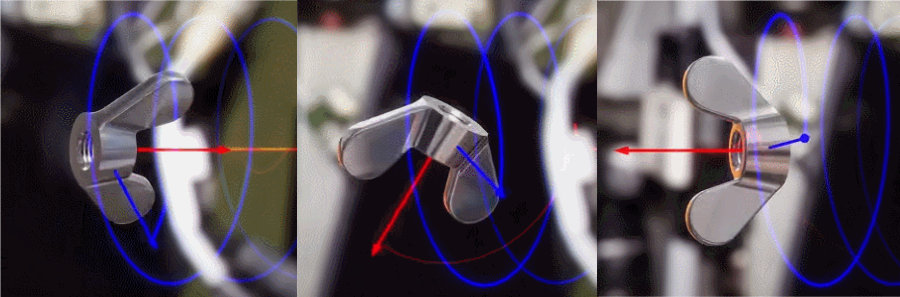
\includegraphics[width=0.9\textwidth]{dzhani.jpg}
\end{center}
   \caption{Eine Darstellung des Dschanibekow-Effekts \cite{28}.}
\label{fig:10}
\end{figure*}

Das Prinzip hinter einer schnellen Veränderung der Rotationsachse der Erde liegt in der Physik rotierender Objekte. Das klassische Beispiel dafür ist der Dschanibekow-Effekt, entdeckt vom russischen Kosmonauten Wladimir Dschanibekow \cite{37}, und in Abbildung \ref{fig:10} dargestellt. Ein Objekt, das sich nicht perfekt um eine seiner drei Hauptträgheitsachsen dreht, wird seine Rotationsachse nicht beibehalten. Wenn es sich nahe der zweiten Hauptträgheitsachse dreht, wird es scheinbar plötzliche Veränderungen der Rotation erfahren. Auch wenn dies nicht genau das ist, was wir bei den schnellen Umkehrungen der Erde vermuten, ist der Punkt, dass im Fehlen äußerer Kräfte nur die Rotationsphysik einen schnellen Wechsel der Rotationsachse der Erde erklären kann.

Genauer gesagt erfährt die Erde mit großer Sicherheit keinen einfachen und gleichmäßigen Dschanibekow-Effekt. Wenn dies der Fall wäre, könnten wir über die Zeit eine allmähliche Verschiebung der Rotationsachse der Erde feststellen. Stattdessen wird angenommen, dass die Erde periodisch plötzliche Störungen in ihrer physikalischen Struktur erlebt, was zu einer Entkopplung ihrer "äußeren Rotationskörper" (Kruste/Mantel) und "inneren Rotationskörper" (Kern) führt. Ohne einen äußeren Impuls besagt das Gesetz der Erhaltung des Drehimpulses, dass die Erde ihre Rotationsachse nicht plötzlich verändern kann, sodass eine Entkopplung zwischen äußeren und inneren Rotationskörpern eine der wenigen Ursachen wäre, abgesehen von einem externen Einschlag, die eine schnelle und abrupte Umkehr verursachen könnte.

Der spezifische Prozess, der die interne Störung in der Erde antreibt, wird als Phasenübergang in der Struktur des Eisens angesehen, das den Erdkern bildet (Abbildung \ref{fig:11}). Der innere Kern besteht aus hexagonal dichtest gepacktem Eisen (Fe) \cite{141}. Wenn dieses hcp-Fe in einen flüssigen metallischen Zustand übergeht, wird kinetische Energie freigesetzt und in den äußeren Kern ausgestoßen. Dieser Phasenwechsel verringert die magnetische Permeabilität des Kerns, schwächt das geomagnetische Feld und setzt Wärme frei, wodurch LLVP-Strukturen (large low-velocity shear province, große Gebiete mit niedriger Schergeschwindigkeit) (Abbildung \ref{fig:12}) \cite{38} im Mantel entstehen und die Erdoberfläche durch die abyssalen Ozeane erhitzt wird. Beide Entwicklungen sind in den letzten Jahrhunderten gut dokumentiert und werden später in dieser Arbeit behandelt.

\begin{figure*}[t]
\begin{center}
% \fbox{\rule{0pt}{2in} \rule{.9\linewidth}{0pt}}
\includegraphics[width=1\textwidth]{layers.jpg}
\end{center}
   \caption{Darstellung der inneren Erdprozesse, die zum ECDO-Flip führen \cite{129}.}
\label{fig:11}
\end{figure*}
\begin{figure}[t]
\begin{center}
% \fbox{\rule{0pt}{2in} \rule{0.9\linewidth}{0pt}}
   \includegraphics[width=1\linewidth]{llvp.jpg}
\end{center}
   \caption{Eine detaillierte Darstellung des LLVP unter Südafrika \cite{28}.}
\label{fig:12}
\label{fig:onecol}
\end{figure}


Dieser gleiche Prozess im Inneren der Erde, der in umgekehrter Weise abläuft, soll auch den Wechsel zurück zum aktuellen Rotationszustand der Erde relativ kurz nach dem Umpolen antreiben.

\section{Beweise für eine bevorstehende Erdumkehr}

Es gibt starke Gründe zu glauben, dass wir am Rande einer weiteren Erdumkehr stehen. Eine Katastrophe hat seit mehreren Jahrtausenden nicht stattgefunden, was ungefähr der Häufigkeit entspricht, mit der diese Ereignisse laut historischen Berichten und Daten aufzutreten scheinen. Die stärksten Daten zur Unterstützung einer bevorstehenden Umkehr stammen von aktuellen geomagnetischen Messungen, die darauf hindeuten, dass das geomagnetische Feld der Erde seit etwa zweitausend Jahren schwächer wird. Diese Abschwächung hat sich beschleunigt und in den letzten Jahrzehnten beunruhigende Werte erreicht.

Abgebildet in Abbildung \ref{fig:14} ist das geomagnetische Feld der Erde in den Jahren 1590 und 2025 \cite{125,126}. Wie in der Abbildung gezeigt, hat sich das Feld deutlich abgeschwächt.
Ein weiteres Maß für das schwächer werdende geomagnetische Feld ist die Position des geomagnetischen Nordpols (Abbildung \ref{fig:13}). Der geomagnetische Nordpol befand sich historisch im kanadischen Arktisgebiet. Allerdings ist er in den letzten Jahrhunderten langsam gewandert und hat sich vor einigen Jahrzehnten deutlich beschleunigt. Er bewegt sich nun mit einer Geschwindigkeit von 55 Kilometern pro Jahr rasch in Richtung Russland \cite{124}.

\begin{figure*}[t]
\begin{center}
% \fbox{\rule{0pt}{2in} \rule{.9\linewidth}{0pt}}
\includegraphics[width=0.9\textwidth]{saa.jpg}
\end{center}
   \caption{Eine Darstellung des sich abschwächenden geomagnetischen Feldes von 1590 bis 2025. Berechnet mit den Modellen gufm1 und IGRF-14 \cite{125,126}.}
\label{fig:14}
\end{figure*}

\begin{figure}[t]
\begin{center}
% \fbox{\rule{0pt}{2in} \rule{1\linewidth}{0pt}}
   \includegraphics[width=1\linewidth]{npw.jpg}
\end{center}
   \caption{Die Position des geomagnetischen Nordpols von 1590 bis 2025, dargestellt in 5-Jahres-Schritten \cite{142}.}
\label{fig:13}
\label{fig:onecol}
\end{figure}

\begin{figure}[t]
\begin{center}
% \fbox{\rule{0pt}{2in} \rule{1\linewidth}{0pt}}
   \includegraphics[width=1\linewidth]{ocean-highlight.jpg}
\end{center}
   \caption{Erwärmungsraten im tiefen Ozean ($>$2000 m Tiefe) von 1991 bis 2010, rot umkreist \cite{132}.}
\label{fig:15}
\label{fig:onecol}
\end{figure}

Es wird angenommen, dass das Magnetfeld der Erde von einem inneren Dynamo erzeugt wird – zirkulierende Magmasäulen, die sich aufgrund der Erdrotation im äußeren Erdkern bewegen \cite{123}. Ein abgeschwächtes geomagnetisches Feld ist ein Symptom für Störungen tief im Erdinneren. Laut der ECDO-Theorie stoßen diese Störungen Wärme aus und führen schließlich zur Entkopplung von Mantel und Kern, was eine Umkehr der Erde verursacht \cite{1}.

Es gibt zahlreiche Daten, die das Vorhandensein exothermer Prozesse im Erdinneren bestätigen. Eine Erwärmung der Erde wird durch steigende kontinentale und ozeanische Oberflächentemperaturen dokumentiert \cite{127,128}, durch zunehmende atmosphärische CO2-Werte, die im Einklang mit den Wärmeströmen der Erde schwanken \cite{129,130}, und durch eine Abnahme der globalen Meereisausdehnung \cite{131}. Die Daten deuten darauf hin, dass steigende CO2-Werte und Temperaturen nicht die Ursache des "menschenverursachten" Klimawandels sind, sondern vielmehr nachgelagerte Effekte eines exothermen Erdkerns \cite{129}.

Am bedeutendsten ist, dass Untersuchungen der Erwärmungsraten im tiefen Ozean (Tiefe $>$2000 Meter) zeigen, dass nicht nur die Tiefsee sich erwärmt, sondern die stärksten Erwärmungsraten in der abyssalen Schicht (4000–6000 m) zu finden sind. Diese Erwärmung der Tiefsee hat ihr Zentrum unterhalb von 4000 Metern \cite{132,129}, was nicht möglich wäre, wenn die Ozeane von oben durch die Atmosphäre erwärmt würden. Solche Daten stützen nachdrücklich die Annahme, dass aktuelle Klima- und geomagnetische Veränderungen durch Prozesse tief im Erdinneren verursacht werden. Abbildung \ref{fig:15} zeigt die globalen Erwärmungsraten des Tiefseeozeans von 1991 bis 2010 \cite{132}.

\section{Modellierung der bevorstehenden Erdumkehrung}
\begin{figure}[b]
\begin{center}
% \fbox{\rule{0pt}{2in} \rule{1\linewidth}{0pt}}
   \includegraphics[width=1\linewidth]{saa-crop.jpeg}
\end{center}
   \caption{Eine Kipppunktberechnung basierend auf der Südatlantischen Anomalie weist auf ein Datum vom 13. März 2059 hin \cite{125,126}.}
\label{fig:16}
\label{fig:onecol}
\end{figure}

Die Vorhersage des Zeitpunkts der nächsten Umpolung der Erde ist eine komplexe Aufgabe. Das derzeit beste Modell hierfür liegt im geomagnetischen Feld der Erde – der Südatlantischen Anomalie (SAA). Diese Region über dem Südatlantik weist die schwächste geomagnetische Feldstärke auf und ist als das Gebiet definiert, dessen Feldstärke unter 32.000 Nanotesla liegt \cite{135}, was 1590 der niedrigste Feldwert war. Die Fläche der Südatlantischen Anomalie nahm von 1\% der Erdoberfläche im Jahr 1590 auf 21\% im Jahr 2025 zu \cite{136}.

Um eine Schätzung dafür zu erhalten, wann die Erde umkippen könnte, habe ich die Flächenausdehnung der SAA mit einer Potenzgesetz-Kipppunkt-Gleichung angepasst, die ein komplexes System modelliert, das sich einer kritischen Transition nähert, bei der das System einen dramatischen und abrupten Wandel durchläuft. Meine Berechnungen ergaben ein vorhergesagtes Kipppunkt-Datum vom 13. März 2059 (Abbildung \ref{fig:16}). Diese Vorhersage wird umso genauer, je näher wir dem Übergang kommen \cite{136}.

Weitere Kennzahlen wie das Wandern der Rotationsachse, Wetteranomalien sowie seismische und vulkanische Daten können ebenfalls helfen, eine bessere Vorhersage darüber zu treffen, wann die nächste Erdpolumkehr eintreten könnte.

\section{ECDO Historische Zeitleiste}

Auch wenn es schwierig ist, eine genaue Zeitleiste für vergangene ECDO-Ereignisse aufzustellen, scheint es zumindest 2 ECDO-Ereignisse während des Holozäns gegeben zu haben. Beachten Sie den Bericht, den Herodot von ägyptischen Priestern überliefert, dass \textit{"vom ersten König bis zu diesem Priester des Hephaistos, der zuletzt regierte, es dreihunderteinundvierzig Generationen von Menschen gegeben habe... In dieser Zeit, so sagten sie, habe die Sonne viermal ihren gewohnten Aufgangspunkt verlassen, und wo sie jetzt untergeht, sei sie zweimal aufgegangen, und an dem Ort, an dem sie jetzt aufgeht, sei sie zweimal untergegangen"} \cite{32}. Platon, der im fünften Jahrhundert v. Chr. lebte \cite{111}, erklärte, dass nach der Flut, die Atlantis in einer einzigen Nacht und einem Tag vor 9.000 Jahren versenkte, \textit{"seitdem viele Überschwemmungen stattgefunden haben, und die Überlebenden in den Bergen keine Kenntnis der Schrift hatten und sich über viele Generationen hinweg ganz dem Erwerb der notwendigen Mittel zum Leben widmeten"} \cite{112}, was darauf hindeutet, dass es seit dem Ende des Jüngeren Dryas um 9700 v. Chr. mehr als zwei Umpolungen gegeben hat. Die in dieser Arbeit und in meinen Forschungen angeführten physischen Belege \cite{2} bieten reichlich Hinweise für Platons Darstellung.

Die jüngste Kandidatendatum für einen ECDO-Flip liegt im Zeitraum von 2300 bis 1600 v. Chr., auf den viele katastrophale Flutberichte (Gun-Yu \cite{113,114,115}, Ogyges \cite{116,117}, Peru \cite{118,119}, Exodus \cite{120}), Zerstörungen und Aufgabe von Zivilisationen (Mohenjo-Daro \cite{121}, minoisches Kreta\cite{100,101}) und physikalische Anomalien (Bond-Ereignisse \cite{122}, 4,2-Kilojahr-Ereignis \cite{90}) datiert sind. Es gibt keine ausreichende Übereinstimmung von Beweisen, die jünger sind als dieses Datum und auf ein großes katastrophales Ereignis hindeuten.

\section{Fazit}

Operation NANOOK war eine Aufklärungsmission der Vereinigten Staaten im Kalten Krieg, um nach dem Zweiten Weltkrieg die Arktis und die nördliche Sowjetküste zu kartieren \cite{137}. Während ihrer Untersuchung stellten sie fest, dass der magnetische Pol 125 bis 200 Meilen nördlich von dem lag, wo er laut früheren Expeditionen sein sollte. Dementsprechend \textit{"kam unter den Regierungswissenschaftlern die Frage auf, was passieren würde, wenn der magnetische und der geografische Pol zusammenfallen würden. Um dies zu beantworten, wurde unter der Projektleitung von Dr. Paul A. Siple die Rand Corporation beauftragt, Laborexperimente durchzuführen, bei denen Modelle der Erde aus konzentrischen Kugeln verwendet wurden – eine innere Kugel stellte den elektromagnetisch aufgeladenen, geschmolzenen Eisenkern der Erde dar, dessen Achse die „magnetischen“ Pole bestimmte; und eine äußere Kugel stellte die Erdkruste dar, die sich um eine „geografische“ Polachse drehte. Durch wiederholte Experimente wurde festgestellt, dass, während sich der „magnetische“ Pol dem „geografischen“ Pol näherte, der „magnetische“ Pol irgendwann seine Annäherungsgeschwindigkeit beschleunigen würde, als ob er durch Zentripetalkraft zum „geografischen“ Pol gezogen würde und mit diesem zusammenfällt; aber anstatt dass die Pole zusammenfallen, würde der „magnetische“ Pol schnell um den „geografischen“ Pol „flippen“ und dann wie durch Zentrifugalkraft in Richtung Äquator schleudern, wobei er an einer Position landet, an der die beiden Achsen ungefähr einen 89-Grad-Winkel bilden. Nachdem dieser polare „Flip“ stattgefunden hatte, würden sich die Achsen über einen langen Zeitraum hinweg wieder allmählich annähern."} \cite{138,139}

Anschließend \textit{"bei einem der wissenschaftlichen Treffen, an denen Major White Anfang 1948 im Pentagon teilnahm, diskutierten die Wissenschaftler die Zweckmäßigkeit, die Öffentlichkeit auf das bevorstehende Polsprung-Phänomen aufmerksam zu machen. Keiner der Wissenschaftler war bereit, die Information der Öffentlichkeit vorzuenthalten; aber andererseits konnte sich auch niemand einigen, wie man sie veröffentlichen sollte. Das Wissen um dieses Phänomen, so meinten einige, könnte an sich bereits das moralische Gefüge der Gesellschaft zerstören. Ihre Ängste erwiesen sich offenbar als unbegründet, als Anfang der 1950er Jahre Informationen über das Flip-Phänomen sowohl in einer Zeitungsspalte als auch in einem Zeitschriftenartikel veröffentlicht wurden, aber überraschenderweise keinerlei Reaktionen einer offenbar verblüfften, provinziellen oder ungläubigen Öffentlichkeit auslösten."} \cite{138,139}

Warum schenken wir dem keine Beachtung? Es gibt genügend Gründe zu der Annahme, dass sich die Erde schon früher gedreht hat. Diese Arbeit, zusammen mit dem zweiten Teil, bietet eine umfassende Zusammenfassung einer großen Konvergenz von Beweisen aus vielen Bereichen, die darauf hindeuten, dass dies der Fall ist, wie Flutgeschichten aus aller Welt, Salz- und Meeresfossilien, die die Kontinente bedecken, uralte unterirdische Schutzräume, Tierüberreste und katastrophale geologische Landschaften. Der Mensch gilt als Hunderttausende von Jahren alt, und doch reicht die moderne Geschichte nur einige tausend Jahre zurück. Könnte es nicht sein, dass die Erde von Zeit zu Zeit kippt, die Kontinente ausgelöscht werden und wir gezwungen sind, zum Ausgangspunkt zurückzukehren – ins Steinzeitalter – und damit die Aufzeichnungen der alten Geschichte auf eine Handvoll katastrophaler Geschichten reduziert werden? Wenn dem so ist, könnte es eine der wichtigsten Aufgaben der Menschheit sein, dies künftig zu verhindern.

Abschließend möchte ich Ihnen diesen Bericht aus dem Timaios von Platon hinterlassen, der von einem Gespräch zwischen Solon, einem athenischen Staatsmann, und ägyptischen Priestern erzählt \cite{140}: \textit{"Und als [Solon] sie einmal zu einer Rede über die uralte Geschichte bewegen wollte, versuchte er, ihnen die ältesten unserer Überlieferungen zu erzählen, über Phoroneus, der als der erste Mensch galt, und Niobe; und er fuhr fort, die Sage über Deukalion und Pyrrha nach der Flut zu berichten und wie sie diese überlebten, und die Genealogie ihrer Nachkommen zu geben; und indem er die Zahl der von den genannten Ereignissen eingenommenen Jahre aufzählte, versuchte er die Zeitabschnitte zu berechnen. Da sagte einer der Priester, ein ungemein alter Mann: „O Solon, Solon, ihr Griechen seid immer Kinder: Es gibt so etwas wie einen alten Griechen nicht.“ Nachdem er das gehört hatte, fragte er: „Was meinst du mit diesem Spruch?“ Und der Priester antwortete: „Ihr seid alle jung an der Seele. Denn darin besitzt ihr keinen einzigen Glaubenssatz, der alt ist und aus alter Überlieferung stammt, noch eine Wissenschaft, die mit dem Alter verwittert ist. Und das ist der Grund: Es gab und wird viele und unterschiedliche Zerstörungen der Menschheit geben, von denen die größten durch Feuer und Wasser, die kleineren durch zahllose andere Mittel geschehen. Denn tatsächlich ist die Geschichte, die sowohl in eurer als auch in unserer Heimat erzählt wird, wie einst Phaethon, der Sohn des Helios, den Wagen seines Vaters anspannte und, weil er ihn nicht im Lauf des Vaters führen konnte, alles auf der Erde verbrannte und selbst durch einen Blitz ums Leben kam – diese Geschichte hat zwar das Gepräge einer Sage, aber der wahre Kern liegt in der Verschiebung der Himmelskörper, die um die Erde kreisen, und in der Zerstörung der Dinge auf der Erde durch gewaltiges Feuer, das in langen Abständen wiederkehrt. Zu solchen Zeiten werden alle, die in den Bergen und in hohen, trockenen Gegenden leben, mehr vernichtet als jene, die in der Nähe von Flüssen oder dem Meer wohnen; und bei uns rettet uns der Nil, unser Retter auf andere Weise, auch in solchen Zeiten vor diesem Unglück, indem er hoch ansteigt. Wenn aber umgekehrt die Götter die Erde mit einer großen Flut reinigen, werden alle Hirten und Schäfer in den Bergen gerettet, während die in euren Städten durch die Strömungen ins Meer gespült werden; in unserem Land aber strömt das Wasser weder dann noch sonst zu irgendeiner Zeit von oben auf unsere Felder herab, im Gegenteil, es quillt immer von unten herauf. Deshalb wird aus diesen Gründen das, was hier erhalten geblieben ist, als das älteste betrachtet; in Wirklichkeit existiert an jedem Ort, wo nicht übermäßige Hitze oder Kälte die Entstehung verhindern, immer eine Art Menschengeschlecht, mal mehr, mal weniger zahlreich. Und wenn irgendein Ereignis stattgefunden hat, das vornehm oder groß oder in irgendeiner Weise auffällig ist, gleichviel ob es in eurem Land oder unserem oder in irgendeinem anderen Ort, von dem wir durch Überlieferung wissen, war, so werden alle solche Ereignisse von alters her aufgezeichnet und in unseren Tempeln erhalten; während eure Leute und die anderen jedes Mal aufs Neue nur mit Buchstaben und all den Künsten ausgestattet werden, die kultivierte Staaten benötigen, und wenn nach dem üblichen Zeitabstand, wie eine Seuche, die Flut vom Himmel über euer Volk hereinbricht, bleibt von euch niemand übrig als die Ungebildeten und Unkultivierten, sodass ihr so jung wie zuvor bleibt und nichts wisst, was sich in alten Zeiten in diesem Lande oder in eurem eigenen ereignet hat. Sicher sind die Abstammungslinien, die du eben erzählt hast, Solon, über die Menschen deines Landes, kaum mehr als Kindermärchen; denn erstens erinnerst du dich nur an eine Überschwemmung, obwohl zuvor viele stattgefunden hatten; und dann weißt du nicht, dass das edelste und vollkommenste Menschengeschlecht dort geboren wurde, wo du jetzt wohnst, und von ihnen stammen du selbst und die ganze jetzige Stadt ab, aus einem kleinen Samen, der zufällig übrig geblieben war; das ist dir entgangen, weil viele Generationen lang die Überlebenden keine Möglichkeit hatten, sich schriftlich auszudrücken. Wahrlich, zu einer Zeit, Solon, noch vor der größten Zerstörung durch Wasser, war der heutige athenische Staat der tapferste im Krieg und auch in jeder anderen Hinsicht hervorragend organisiert. Es heißt, er habe die prächtigsten Kunstwerke und die edelste Gesellschaftsordnung aller Völker unter dem Himmel besessen, von denen uns berichtet wurde."}

Diese selben Priester erzählten Solon natürlich auch von der alten Zivilisation Atlantis: \textit{"Alles, was wir hier haben, liegt innerhalb der Mündung, von der wir sprechen, ist erkennbar ein Hafen mit einem schmalen Eingang; dort drüben aber gibt es tatsächlich ein echtes Meer, und das Land, das es umgibt, kann mit vollem Recht, in umfassendstem und wahrstem Sinne, ein Kontinent genannt werden. Nun existierte auf dieser Insel Atlantis eine Konföderation von Königen von großer und wunderbarer Macht, die über die ganze Insel und über viele andere Inseln sowie Teile des Kontinents herrschte; zudem herrschten sie über die Gebiete hier innerhalb der Säulen, über Libyen bis nach Ägypten und über Europa bis nach Tyrrhenien. So versuchte dieses Heer, indem alle zusammenkamen, bei einem einzigen Angriff sowohl euer Land als auch unser sowie das gesamte Gebiet innerhalb der Säulen zu unterwerfen. Und damals, Solon, zeigte sich die Tapferkeit eures Staats im Anblick der ganzen Welt besonders deutlich. Denn er ragte über alle hinaus an Tapferkeit und allen kriegerischen Künsten, und teils als Anführer der Griechen, teils, als er von allen verlassen allein stand, bestand er die tödlichsten Gefahren, besiegte die Angreifer und errichtete ein Siegeszeichen; so bewahrte er jene, die noch nicht versklavt waren, vor der Sklaverei, und alle übrigen, die innerhalb der Grenzen des Herakles wohnten, setzte er großzügig in die Freiheit. Doch später ereigneten sich gewaltige Erdbeben und Überschwemmungen, und ein schlimmer Tag und eine schlimme Nacht trafen sie, als die ganze Streitmacht eurer Krieger von der Erde verschlungen wurde, und die Insel Atlantis ebenso vom Meer verschlungen wurde und verschwand."}

\section{Danksagungen}

Danke an Ethical Skeptic, den ursprünglichen Autor der ECDO-These, für seinen Abschluss dieser aufschlussreichen, bahnbrechenden Arbeit und deren Veröffentlichung. Seine dreiteilige These \cite{1} bleibt das grundlegende Werk zur Exothermic Core-Mantle Decoupling Dzhanibekov Oscillation (ECDO) Theorie und enthält weit mehr Informationen zum Thema, als ich hier kurz dargestellt habe.

Danke an Ankit, der die Katastrophendaten in Tabelle 1 bearbeitet hat.

Und natürlich danken wir den Giganten, auf deren Schultern wir stehen; jenen, die all die Forschung und Untersuchungen durchgeführt haben, die diese Arbeit möglich gemacht haben, und die daran gearbeitet haben, der Menschheit Licht zu bringen.

\clearpage
\twocolumn

\section{Zusätzliche Abbildungen}


\begin{figure}[H]
\begin{center}
% \fbox{\rule{0pt}{2in} \rule{1\linewidth}{0pt}}
   \includegraphics[width=1\linewidth]{wave.jpg}
\end{center}
   \caption{Ein genauer Blick auf die unterschnittene, parabelförmige Wellenerosion an der Chafre-Pyramide \cite{27}.}
\label{fig:19}
\label{fig:onecol}
\end{figure}

\begin{figure}[H]
\begin{center}
\includegraphics[width=1\linewidth]{star-stone.jpg}
\end{center}
   \caption{Die in Stein gemeißelte Sternenkarte in einem der Schächte der Cheops-Pyramide \cite{28}.}
\label{fig:20}
\label{fig:onecol}
\end{figure}

\begin{figure*}[t]
\begin{center}
% \fbox{\rule{0pt}{2in} \rule{.9\linewidth}{0pt}}
\includegraphics[width=1\textwidth]{deepsea.jpg}
\end{center}
   \caption{Eine Darstellung der Tiefsee- und abyssalen Ozean-Erwärmungsanomalie im Vergleich zu einer normalen atmosphärischen Ozeanerwärmungskurve. Die gesamte Erwärmungsanomalie stammt von der NOAA \cite{147}, die Verteilungen der Tiefsee- und Abyssalerwärmung aus einer Studie von Desbruyeres \cite{132}, und die Datenverarbeitung sowie Visualisierung von Ethical Skeptic \cite{129}.}
\label{fig:21}
\end{figure*}

\begin{figure*}[t]
\begin{center}
% \fbox{\rule{0pt}{2in} \rule{.9\linewidth}{0pt}}
\includegraphics[width=1\textwidth]{sealevel.jpeg}
\end{center}
   \caption{Der Meeresspiegel zeigt eine 20\%ige Zunahme der Varianz über 75 Jahre hinweg an 63 Stationen, was auf eine Zunahme der Strömungsgeschwindigkeit hinweist. Anstiege in der Varianz des Meeresspiegels treten gleichzeitig mit ozeanischen Wärmepulsen auf, was darauf hindeutet, dass beide durch eine Erwärmung aus der Tiefe der Ozeane verursacht werden könnten \cite{2,129}.}
\label{fig:22}
\end{figure*}

\begin{figure*}[t]
\begin{center}
% \fbox{\rule{0pt}{2in} \rule{.9\linewidth}{0pt}}
\includegraphics[width=1\textwidth]{co2.jpg}
\end{center}
   \caption{Der atmosphärische CO2-Gehalt in ppm ist in den letzten 45 Jahren kontinuierlich gestiegen, wahrscheinlich verursacht durch einen Anstieg der Meerestemperaturen. Quelle: NOAA \cite{148,129}.}
\label{fig:23}
\end{figure*}

\begin{figure*}[t]
\begin{center}
% \fbox{\rule{0pt}{2in} \rule{.9\linewidth}{0pt}}
\includegraphics[width=1\textwidth]{ice.jpg}
\end{center}

   \caption{Die globale Meereisausdehnung hat in den letzten 45 Jahren aufgrund einer Erwärmung der Erde abgenommen. Quelle: ADS \cite{149}.}
\label{fig:24}
\end{figure*}

\clearpage
\twocolumn

{\small
\renewcommand{\refname}{Verweise}
\bibliographystyle{ieee}
\bibliography{egbib}
}

\end{Dokument}